\documentclass[cs4size,a4paper]{ctexart}
%==================== 中文字体 ============
\setmainfont[Mapping=tex-text]{Times New Roman}
\setsansfont[Mapping=tex-text]{思源黑体 Regular}
\setmonofont{Fira Code}

%% 中文字体
\setCJKmainfont[BoldFont={思源宋体 Bold}, ItalicFont={AR PL UKai CN}]{Source Han Serif SC}
\setCJKsansfont[BoldFont={思源黑体 Bold}]{思源黑体 Regular}
\setCJKmonofont{AR PL UKai CN}       % macos word

\xeCJKsetup{CJKmath=true}
\setCJKmathfont{AR PL UKai CN}  % 数学环境中使用楷体
%==================== 数学符号公式 ============
\usepackage{amsmath}                 % AMS LaTeX宏包
\usepackage[style=1]{mdframed}
\usepackage{amsthm}
\usepackage{amsfonts}
\usepackage{mathrsfs}                % 英文花体字 体
\usepackage{bm}                      % 数学公式中的黑斜体
\usepackage{bbding,manfnt}           % 一些图标,如 \dbend
\usepackage{lettrine}                % 首字下沉,命令\lettrine
\def\attention{\lettrine[lines=2,lraise=0,nindent=0em]{\large\textdbend\hspace{1mm}}{}}
\usepackage{longtable}
\usepackage[toc,page]{appendix}
\usepackage{geometry}                % 页边距调整
\geometry{top=3.0cm,bottom=2.7cm,left=2.5cm,right=2.5cm}
%====================公式按章编号==========================
\numberwithin{equation}{section}
\numberwithin{table}{section}
\numberwithin{figure}{section}
%================= 基本格式预置 ===========================
\usepackage{fancyhdr}
\pagestyle{fancy}
\fancyhf{}
\fancyhead[C]{\zihao{5}  \kaishu 中期检查报告 - 李源勋}
\fancyfoot[C]{~\zihao{5} \thepage~}
\renewcommand{\headrulewidth}{0.65pt}
\CTEXsetup[format={\centering\bfseries\zihao{-2}},name={, }]{section}
\CTEXsetup[nameformat={\bfseries\zihao{3}}]{subsection}
\CTEXsetup[nameformat={\bfseries\zihao{4}}]{subsubsection}
%================== 图形支持宏包 =========================
\usepackage{subfigure}
\usepackage{graphicx}                % 嵌入png图像
\usepackage{color,xcolor}            % 支持彩色文本、底色、文本框等
\usepackage{hyperref}                % 交叉引用
\usepackage{caption}
\usepackage{url}
\usepackage{multirow}
\captionsetup{figurewithin=section}
%==================== 源码和流程图 =====================
\usepackage{listings}                % 粘贴源代码
\usepackage{xcolor}
\usepackage{color}
\definecolor{dkgreen}{rgb}{0,0.6,0}
\definecolor{gray}{rgb}{0.5,0.5,0.5}
\definecolor{mauve}{rgb}{0.58,0,0.82}

%--------------------
\hypersetup{hidelinks}
\usepackage{booktabs}
\usepackage{shorttoc}
\usepackage{tabu,tikz}
\usepackage{float}

\usepackage{multirow}
\usepackage{algorithm}
\usepackage{algorithmicx}
\usepackage{algpseudocode}

\floatname{algorithm}{算法}
\renewcommand{\algorithmicrequire}{\textbf{输入:}}
\renewcommand{\algorithmicensure}{\textbf{输出:}}

\tabcolsep=1ex
\tabulinesep=\tabcolsep
\newlength\tikzboxwidth
\newlength\tikzboxheight
\newcommand\tikzbox[1]{%
        \settowidth\tikzboxwidth{#1}%
        \settoheight\tikzboxheight{#1}%
        \begin{tikzpicture}
        \path[use as bounding box]
                (-0.5\tikzboxwidth,-0.5\tikzboxheight)rectangle
                (0.5\tikzboxwidth,0.5\tikzboxheight);
        \node[inner sep=\tabcolsep+0.5\arrayrulewidth,line width=0.5mm,draw=black]
                at(0,0){#1};
        \end{tikzpicture}%
        }

\makeatletter
\def\hlinew#1{%
  \noalign{\ifnum0=`}\fi\hrule \@height #1 \futurelet
   \reserved@a\@xhline}

\newcommand{\tabincell}[2]{\begin{tabular}{@{}#1@{}}#2\end{tabular}}%

\usepackage{subfigure}
\usepackage{ifthen}


\usepackage{graphicx}
\newcommand{\HRule}{\rule{\linewidth}{0.5mm}}

\newtheorem{Theorem}{定理}
\newtheorem{Lemma}{引理}
%%使得公式随章节自动编号
\makeatletter
\@addtoreset{equation}{section}
\makeatother
\renewcommand{\theequation}{\arabic{section}.\arabic{equation}}

%-------------------------
\usepackage{pythonhighlight}
\usepackage{tikz}
\usepackage{tikz-3dplot}
\usepackage{threeparttable}
\usetikzlibrary{shapes,arrows,positioning}
%===================   正文开始    ===================
\begin{document}
\bibliographystyle{gbt7714-2005}     %论文引用格式
%===================  定理类环境定义 ===================
\newtheorem{example}{例}              % 整体编号
% \newtheorem{algorithm}{算法}
\newtheorem{theorem}{定理}            % 按 section 编号
\newtheorem{definition}{定义}
\newtheorem{axiom}{公理}
\newtheorem{property}{性质}
\newtheorem{proposition}{命题}
\newtheorem{lemma}{引理}
\newtheorem{corollary}{推论}
\newtheorem{remark}{注解}
\newtheorem{condition}{条件}
\newtheorem{conclusion}{结论}
\newtheorem{assumption}{假设}
%==================重定义 ===================
\renewcommand{\contentsname}{目录}
\renewcommand{\abstractname}{摘要}
\renewcommand{\refname}{参考文献}
\renewcommand{\indexname}{索引}
\renewcommand{\figurename}{图}
\renewcommand{\tablename}{表}
\renewcommand{\appendixname}{附录}
\renewcommand{\proofname}{证明}
% \renewcommand{\algorithm}{算法}
%============== 封皮和前言 =================
\begin{titlepage}

\begin{center}


% Upper part of the page

\includegraphics[width=0.65\textwidth]{figure/logo}\\[2cm]

\textsc{\LARGE Xi'an Jiaotong University}\\[1.5cm]

{\Large \textbf{中期检查报告}}\\[0.5cm]


% Title
\HRule \\[0.7cm]
{ \huge \bfseries 面向多CPU集群的深度行人重识别研究}\\[0.4cm]

\HRule \\[1.5cm]

\Large \underline{~电信~}学院~\underline{~计算机~}系~\underline{~44~}班 \\[1cm]

\begin{center}
\begin{Large}
\begin{tabular}{cc}
学生姓名:& 李源勋\\ \cline{2-2}\\
学\qquad 号:&~~~~~2140505083~~~~~\\ \cline{2-2}\\
指导老师:& 何~~晖\\ \cline{2-2}\\
\end{tabular}
\end{Large}
\end{center}

\vfill

% Bottom of the page
{\large \today}

\end{center}

\end{titlepage}

\pagestyle{plain}
\pagenumbering{Roman}

%============== 论文正文   =================
\pagestyle{fancy}
\pagenumbering{arabic}
\section{项目背景及内容}
随着视频监控技术的发展,无人值守的视频监控设备被越来越普遍地部署在国民社会的各个方面,在
公安、交通、智能楼宇、金融、司法、教文卫等领域都有着不可替代的作用。具体的应用场景包括平
安城市、卡口系统、工地监控、自助银行、监狱劳教和学前教育等。

在视频监控领域一个很重要且极具挑战性的问题是行人的重识别。行人重识别,指的是在多个视野不
重叠的监控视频中,重新识别那些之前出现过的行人,即把当前行人与之前已标记的人物相对应。该
工作的实现可以为人物搜索、特定人物跟踪等应用提供强有力的支持,进而应用在平安城市、工地监
控、学前教育等场景。

行人重识别技术在实际应用中受诸多因素的影响,包括摄像头的部署位置、成像质量以及摄像头数量
等等。面对一个从未部署过摄像头的监控场景,一个优秀的摄像头位置部署方案可以实现监控范围无
死角、行人重识别准确率高以及跨摄像头持续跟踪的连续性强。摄像头的成像质量受其自身的性能参
数影响,同时也受部署位置的光线条件影响。在理想情况下,摄像头的数量越多,得到的行人信息就
越多,更有利于行人重识别算法的实施。但是在预算有限的情况下,摄像头的数量不可能无限增加。
因此,如何选择摄像头的数量及其部署位置,使得行人重识别算法的性能最大化,便成为一个极具现
实意义的研究问题。

要实现行人的重识别需要借助计算机视觉领域的技术。目前的计算机视觉算法的前沿关注点主要集中
在深度学习技术。由于深度学习的海量计算需求和GPU强大的并行计算能力,大部分深度学习模型都
是借助GPU来调整模型参数。然而使用GPU进行运算也存在许多问题,例如GPU设备通常比较昂贵,
且少见于嵌入式设备中。同时GPU的显存普遍不高,限制了模型的规模以及每一批次数据的规模。与
此同时,多CPU集群具有硬件成本低、搭建方式灵活以及部署广泛等优点,然而对于深度学习算法在
多CPU集群上的研究与应用少之又少。因此,有必要对深度学习算法在多CPU集群上的性能表现进行
深入的调查、分析和研究。

基于上述研究背景及动机,本项目的主要研究内容和贡献如下:

\begin{enumerate}
\item 深入理解论文\cite{sun2017beyond}的目的、想法和实现方式,并使用PyTorch深度学习框架
复现,达到与原论文接近的实验结果。
\item 研究在预算有限的情况下,摄像头的数量与部署位置对行人重识别算法的影响,并采用强化学习
算法进行摄像头部署位置的选择。
\item 调查、分析和研究深度行人重识别算法在多CPU集群上的性能表现,提出针对多CPU集群环境
的深度神经网络模型的改进策略。
\end{enumerate}

本项目当前的进展:

\begin{enumerate}
\item 搭建了PyTorch分布式环境,完成了论文复现工作,在Market1501\cite{zheng2015scalable}
数据库上进行实验。
\item 实现了 Q-Learning 强化学习算法,选择最优的摄像头部署方案。
\item 将深度行人重识别模型的训练算法改造成适用于多CPU集群的形式。
\end{enumerate}

























      %
\section{项目内容}

\subsection{数据预处理}

    \begin{frame}{数据预处理}
    \begin{block}{}
    \begin{enumerate}
        \item 视频转码
        \item 时间点校正和估计
        \item 视频切割
        \item 行人检测
        \item 人工标注
    \end{enumerate}
    \end{block}
    \begin{figure}
    \centering
    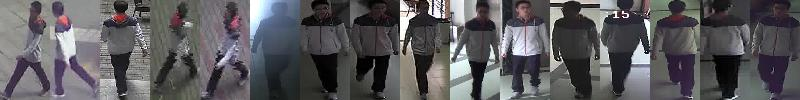
\includegraphics[width=\textwidth]{figures/label}
    \caption{数据预处理的最终结果}
    \label{fig:label}
    \end{figure}
    \end{frame}

    \begin{frame}{行人检测效果}
    \begin{block}{}
    检测视频画面帧中的行人,输出bounding box。
    使用Facebook开源的Detectron工具,其实现了Mask RCNN框架。
    \end{block}
    \begin{figure}
    \centering
    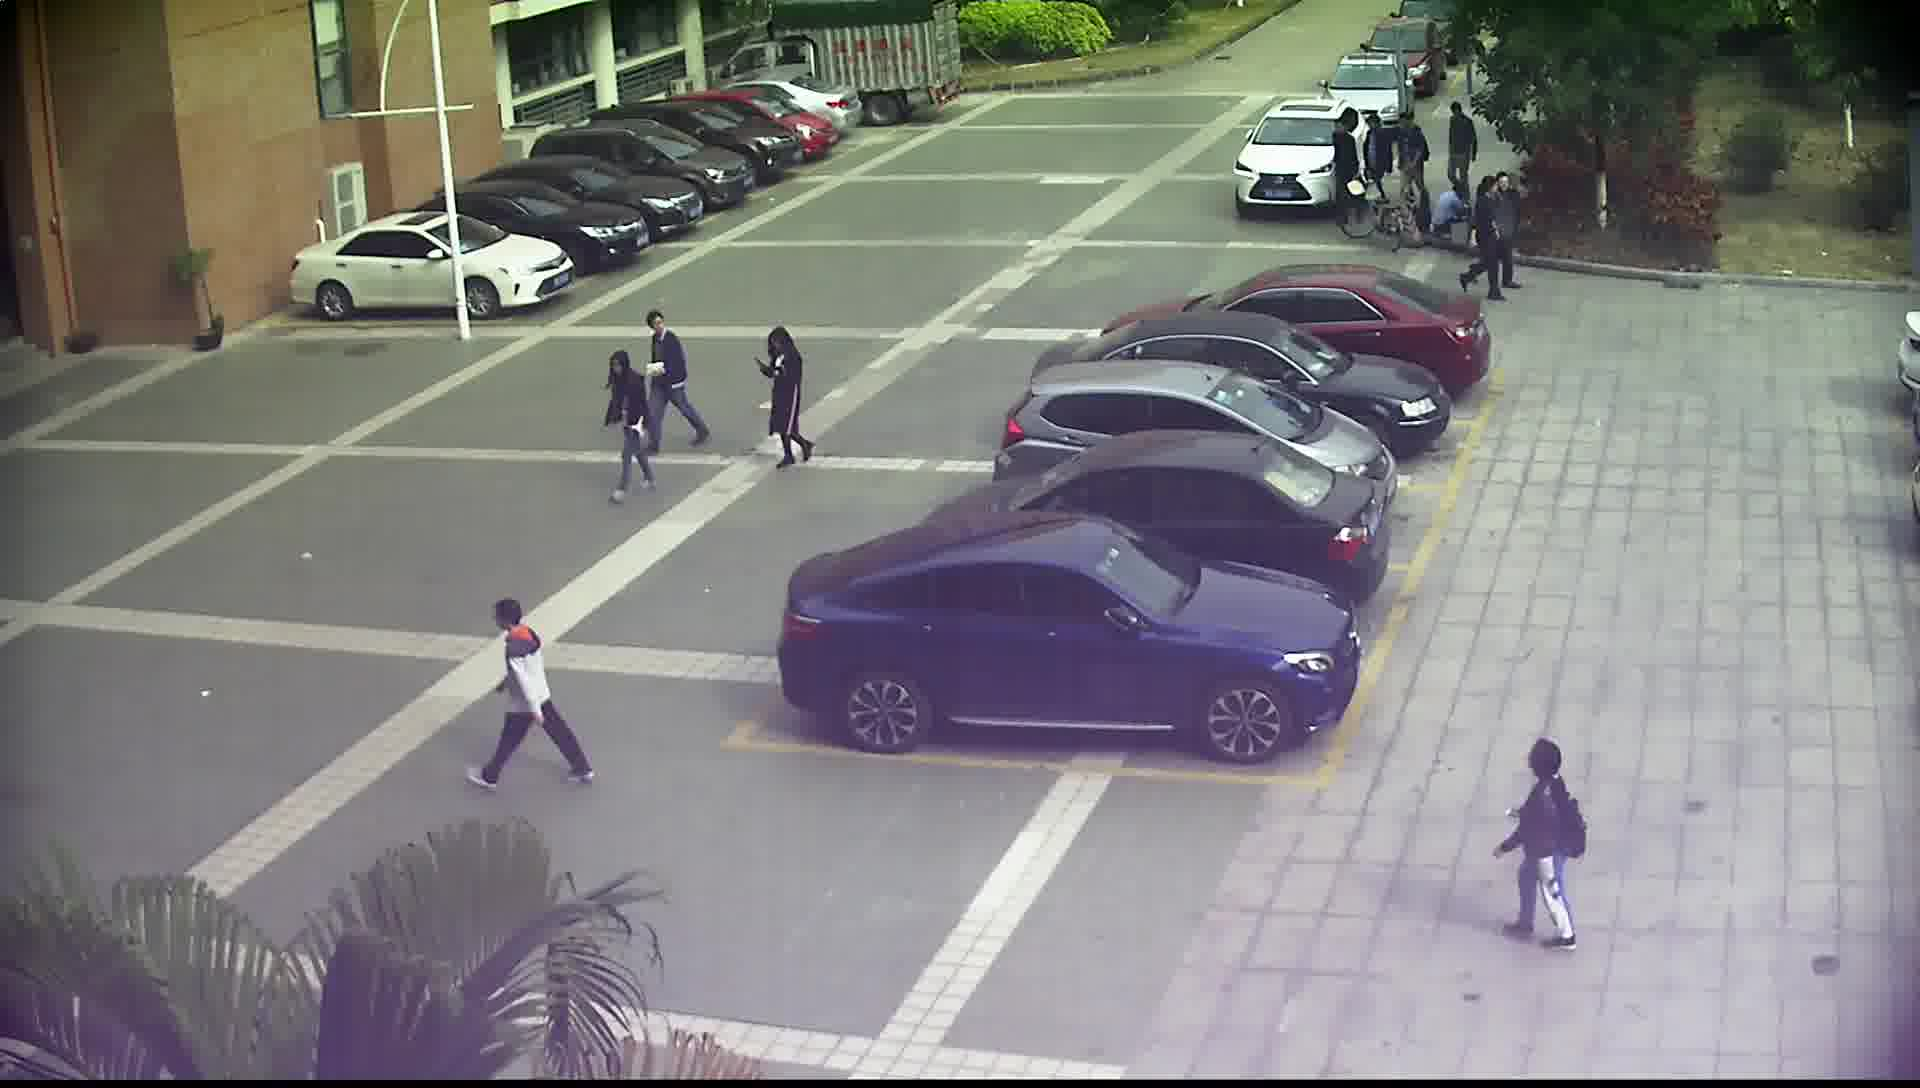
\includegraphics[width=0.3\linewidth]{figures/1-2_5_151.jpg}~
    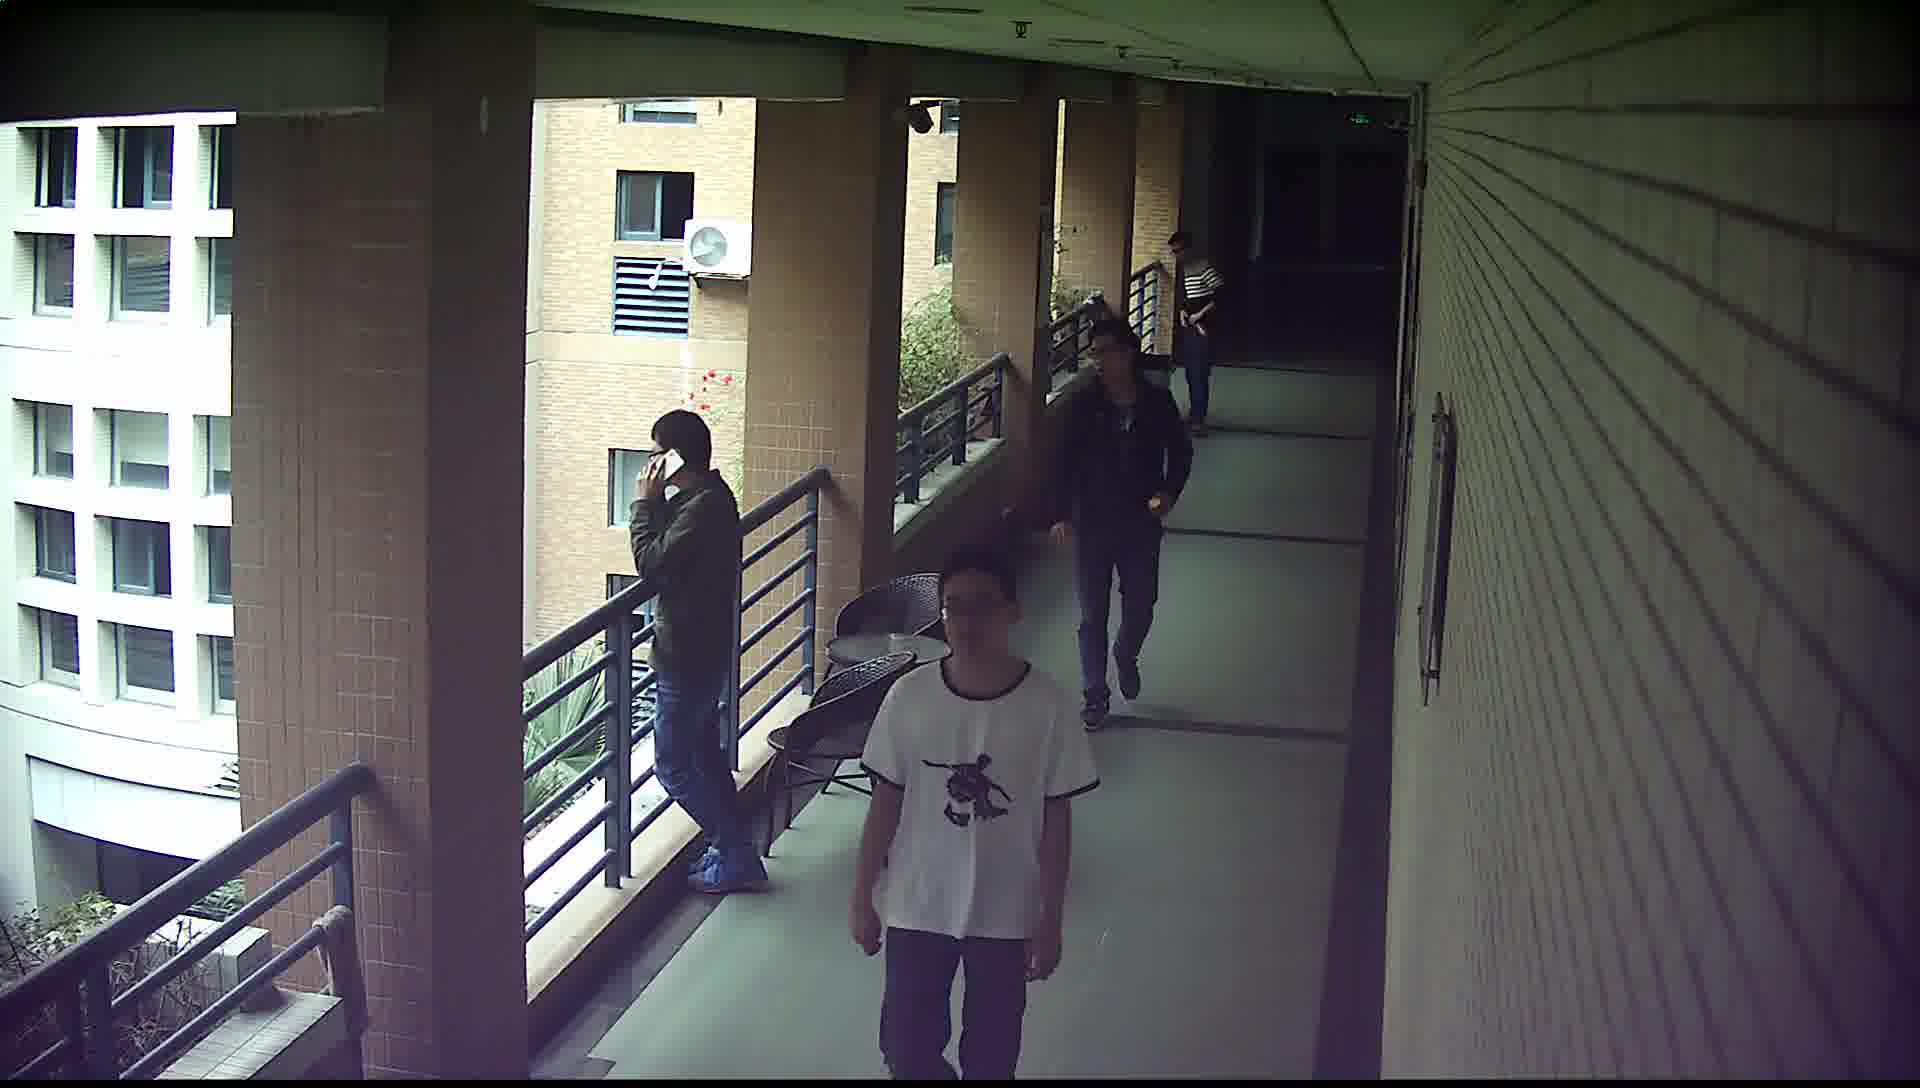
\includegraphics[width=0.3\linewidth]{figures/3-7_10_394.jpg}\\
    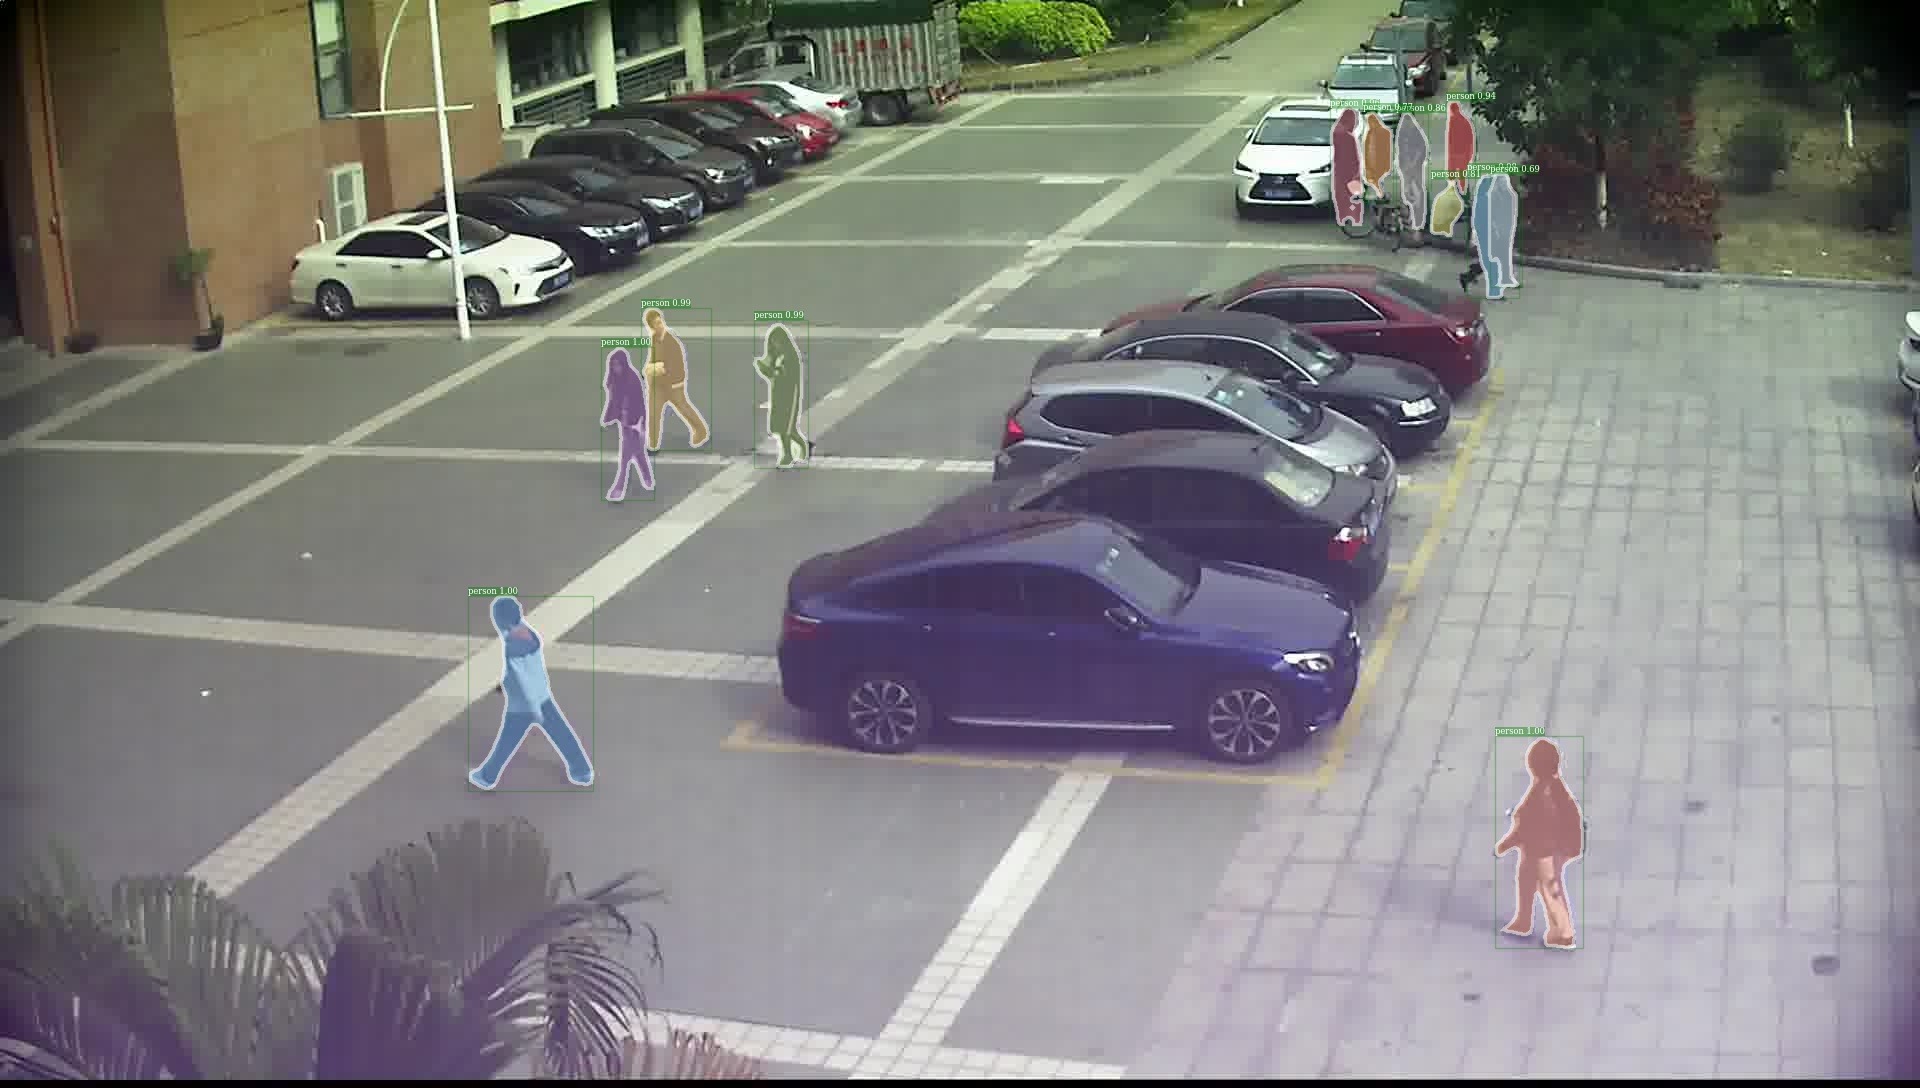
\includegraphics[width=0.3\linewidth]{figures/1-2_5_151_det.jpg}~
    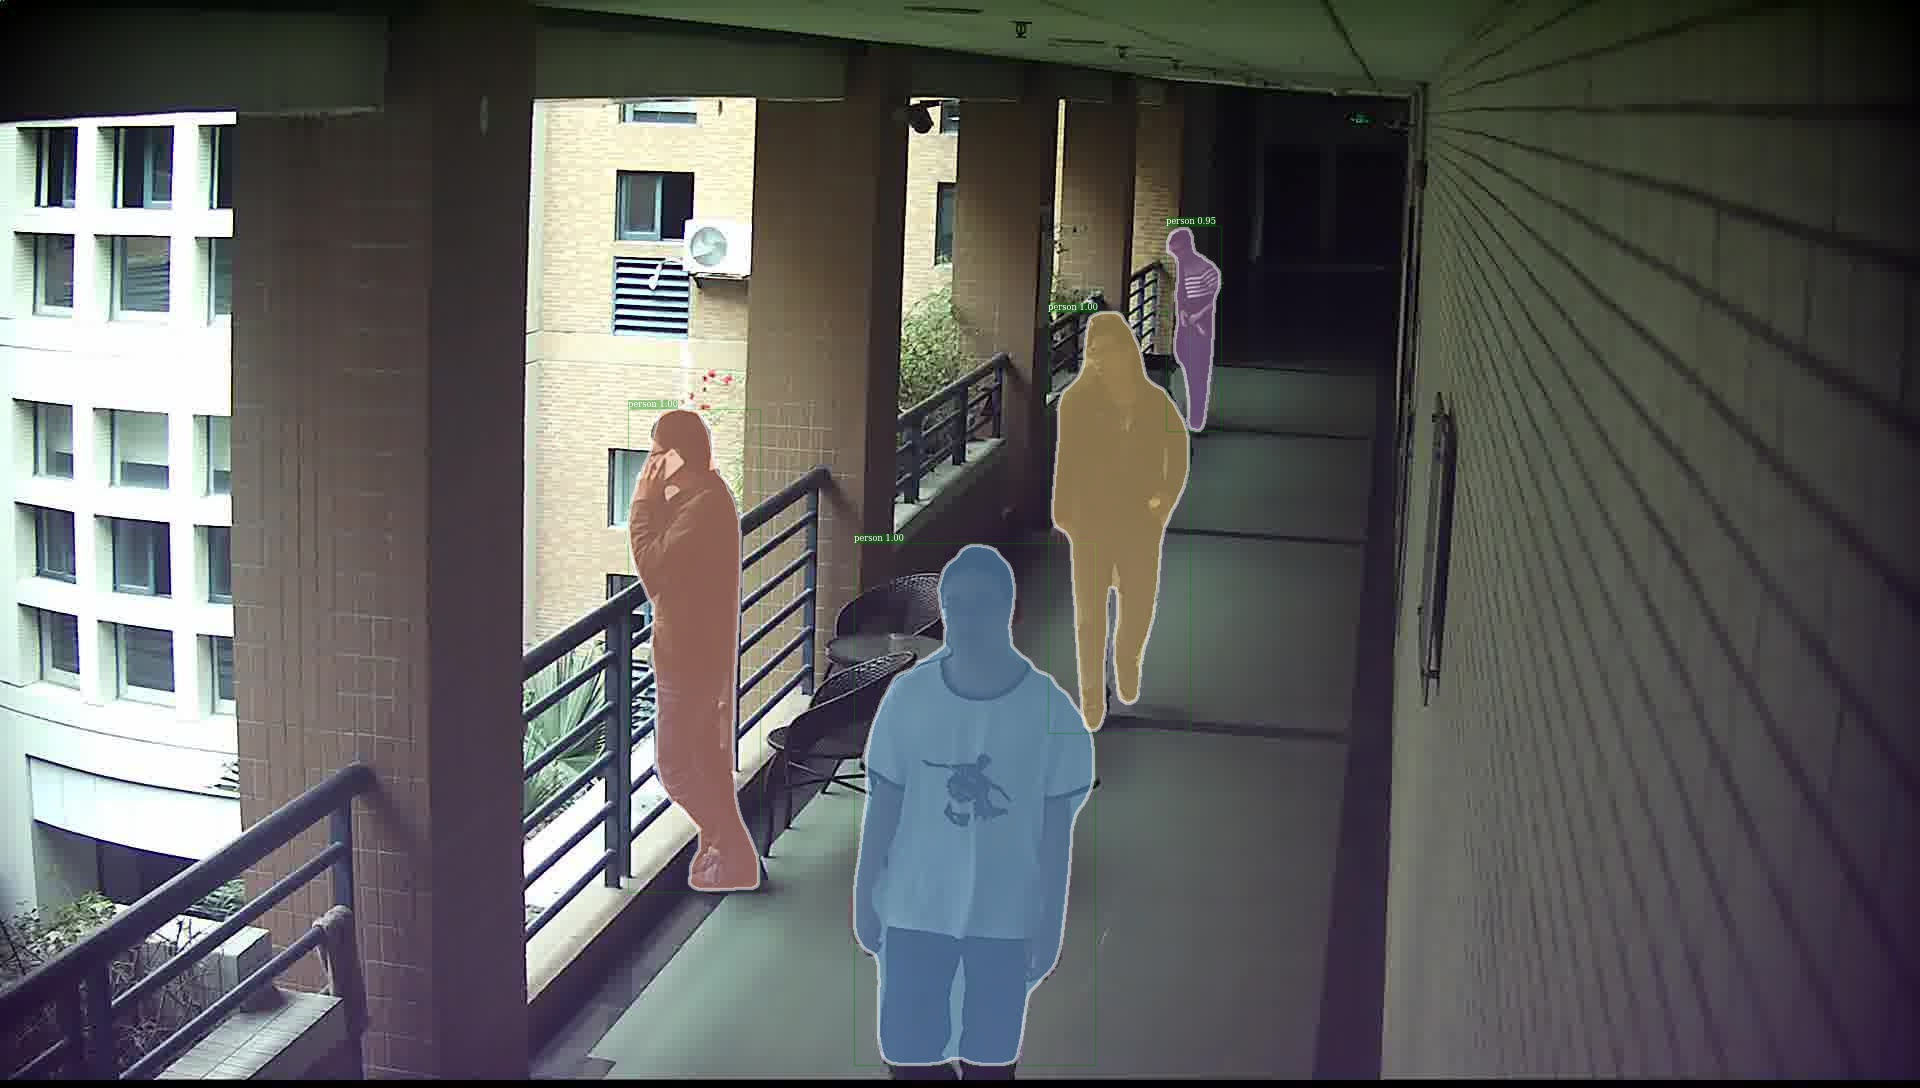
\includegraphics[width=0.3\linewidth]{figures/3-7_10_394_det.jpg}
    \caption{Detectron行人检测结果可视化}
    \label{fig:detectron}
    \end{figure}
    \end{frame}

\subsection{行人重识别论文复现}

    \begin{frame}{行人重识别论文复现结果}
    \begin{block}{}
    训练阶段交叉熵误差(Loss)随着数据集训练批次数(Epoch)变化曲线如图\ref{fig:loss}所示。
    行人重识别,指的是在多个视野不重叠的监控视频中,重新识别那些之前出现过的行人,即把当前行人与之前已标记的人物相对应。
    \end{block}
    \begin{columns}[]
    \centering
    \begin{column}{0.6\textwidth}
        \begin{table}
            \centering
            \begin{tabular}{@{}ccccc@{}}
            \toprule
                    & mAP   & Rank1 & Rank10 \\ \midrule
            论文中显示  & 77.3  & 92.4  & 97.9   \\
            复现结果   & 71.1  & 86.2  & 93.4   \\ \bottomrule
            \end{tabular}
            \caption{Market1501数据集测试结果}
            \label{tab:test}
        \end{table}
    \end{column}
    \begin{column}{0.3\textwidth}
        \begin{figure}[]
            \centering
            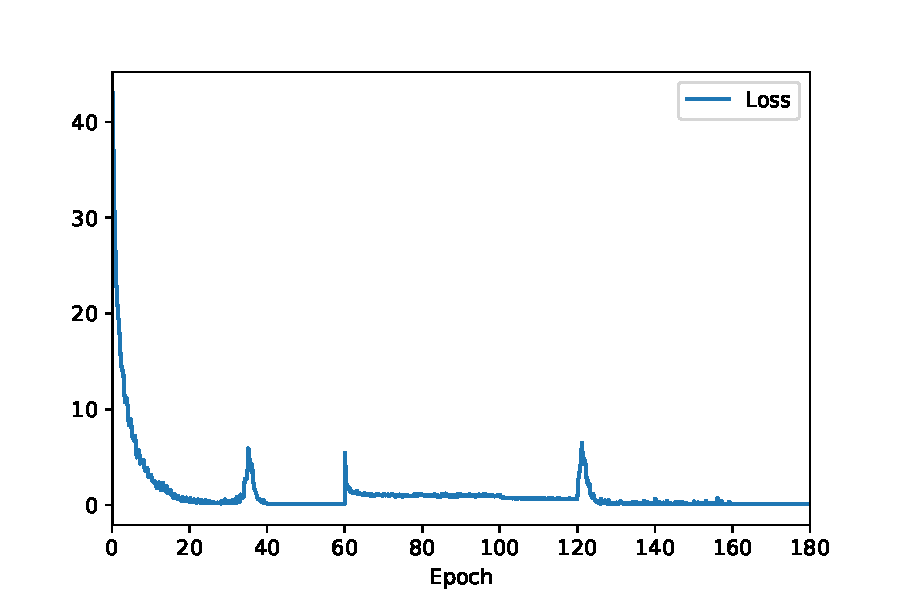
\includegraphics[width=\textwidth]{figures/loss}
            \caption{交叉熵误差随迭代数变化曲线}
            \label{fig:loss}
        \end{figure}
    \end{column}
    \end{columns}
    \end{frame}

    \begin{frame}{测试结果可视化}
        \begin{columns}
            \begin{column}{0.5\textwidth}
                图\ref{fig:testvis}是测试结果的可视化,左边一列是查询图片,每一张查询图片相应的右边一行是从测试库中挑选出来的图片,有红色边框的图片代表该人物标签与相应的查询图片人物标签不一致。
            \end{column}
            \begin{column}{0.5\textwidth}
                \begin{figure}
                \centering
                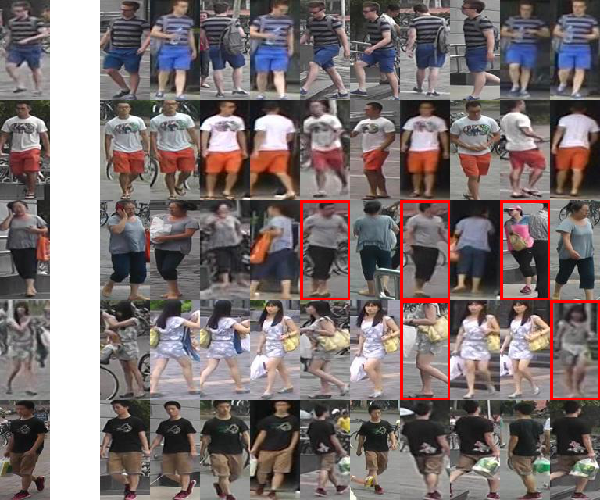
\includegraphics[width=\textwidth]{figures/vis3}
                \caption{测试结果可视化}
                \label{fig:testvis}
                \end{figure}
            \end{column}
        \end{columns}
    \end{frame}

\subsection{强化学习}

    \begin{frame}{经强化学习后选择的部署方案}
    \begin{block}{}
    使用Q-Learning算法,表\ref{tab:rlresult}为经过强化学习训练后的智能体在应对各种状态时,最有可能采取的行动统计。最优方案下的监控画面如图\ref{fig:rlresult}所示。
    \end{block}
    \begin{columns}
        \begin{column}{0.5\textwidth}
            \begin{table}
                \centering
                \begin{tabular}{@{}ccc@{}}
                \toprule
                方案               & 频次  & 占比      \\ \midrule
                (1, 2, 7, 10, 14) & 190 & 65.97\% \\
                (1, 2, 7, 10, 13) & 78  & 27.08\% \\
                (1, 2, 7, 9, 14)  & 18  & 6.15\%  \\
                (1, 3, 7, 10, 14) & 1   & 0.35\%  \\
                (0, 2, 7, 10, 14) & 1   & 0.35\%  \\ \bottomrule
                \end{tabular}
                \caption{学习后选择的部署方案}
                \label{tab:rlresult}
            \end{table}
        \end{column}
        \begin{column}{0.5\textwidth}
            \begin{figure}
            \centering
            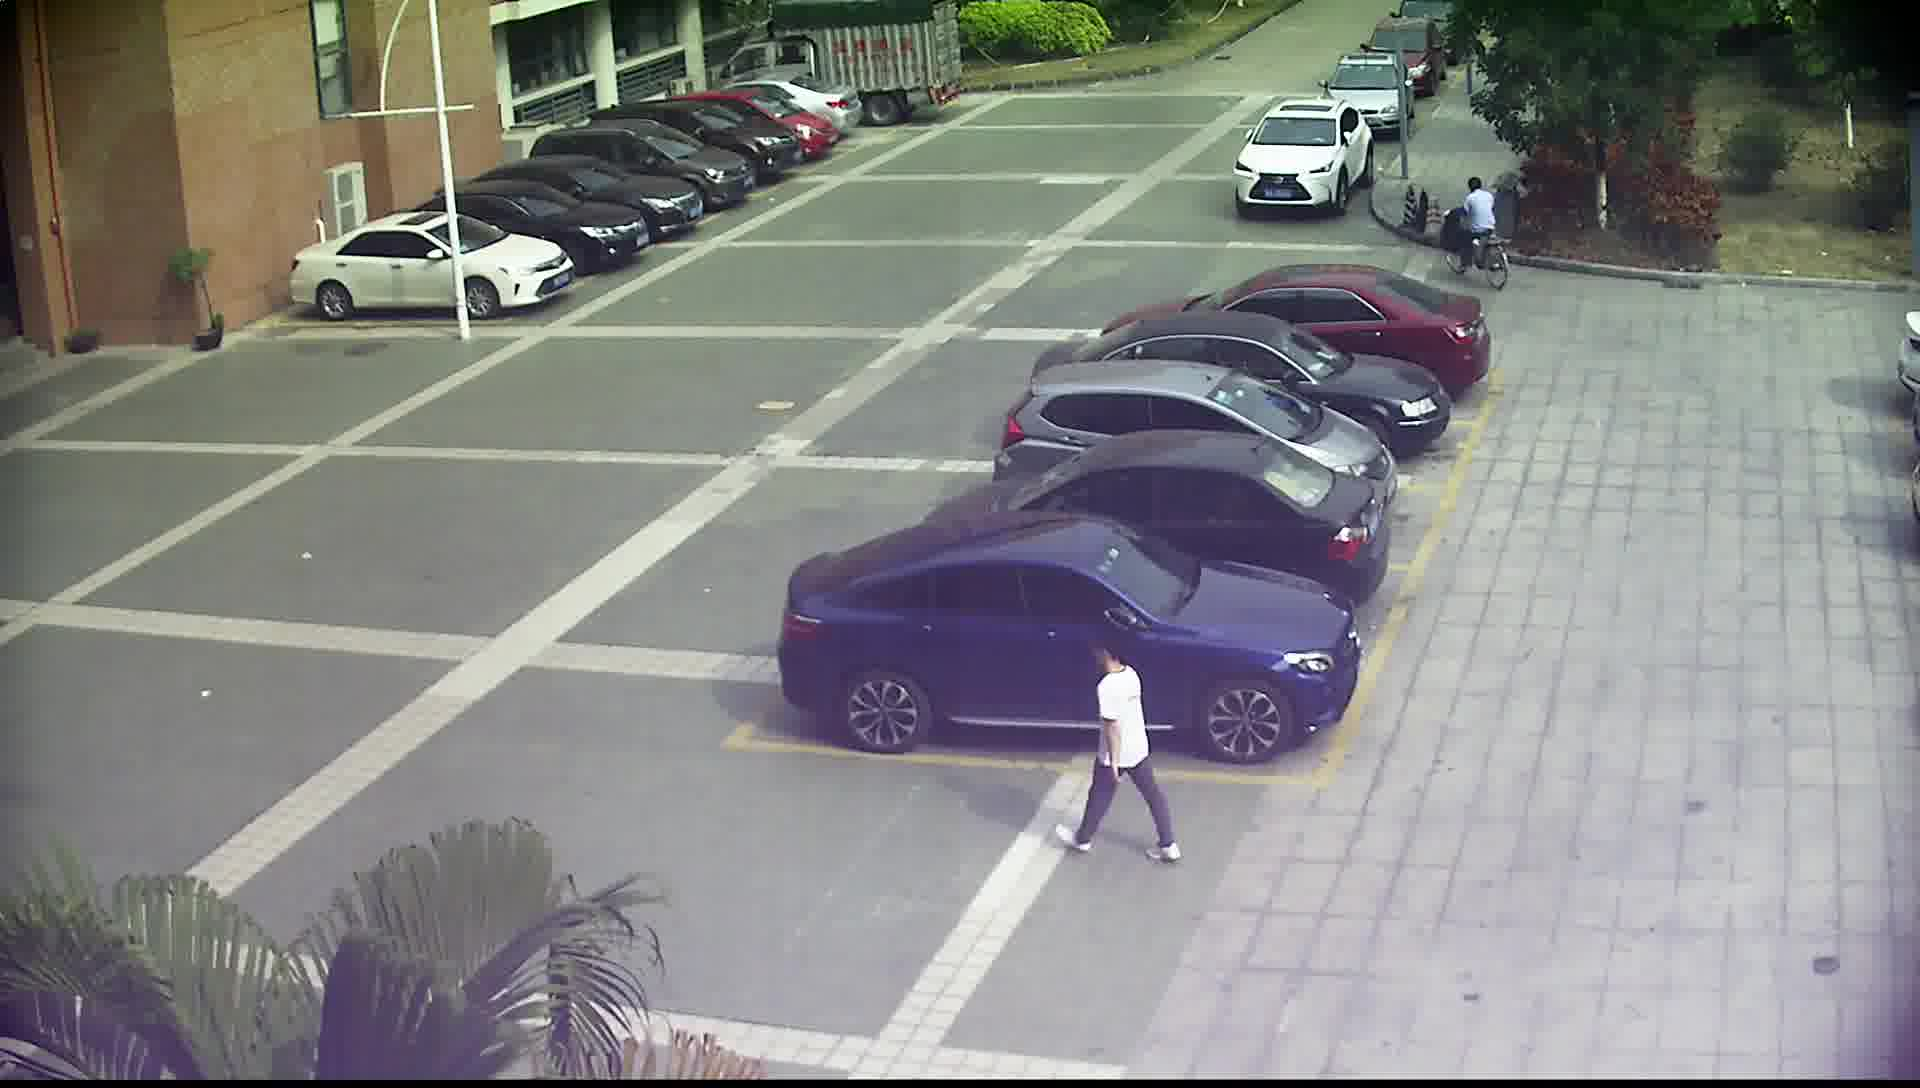
\includegraphics[width=0.3\textwidth]{figures/1-2}
            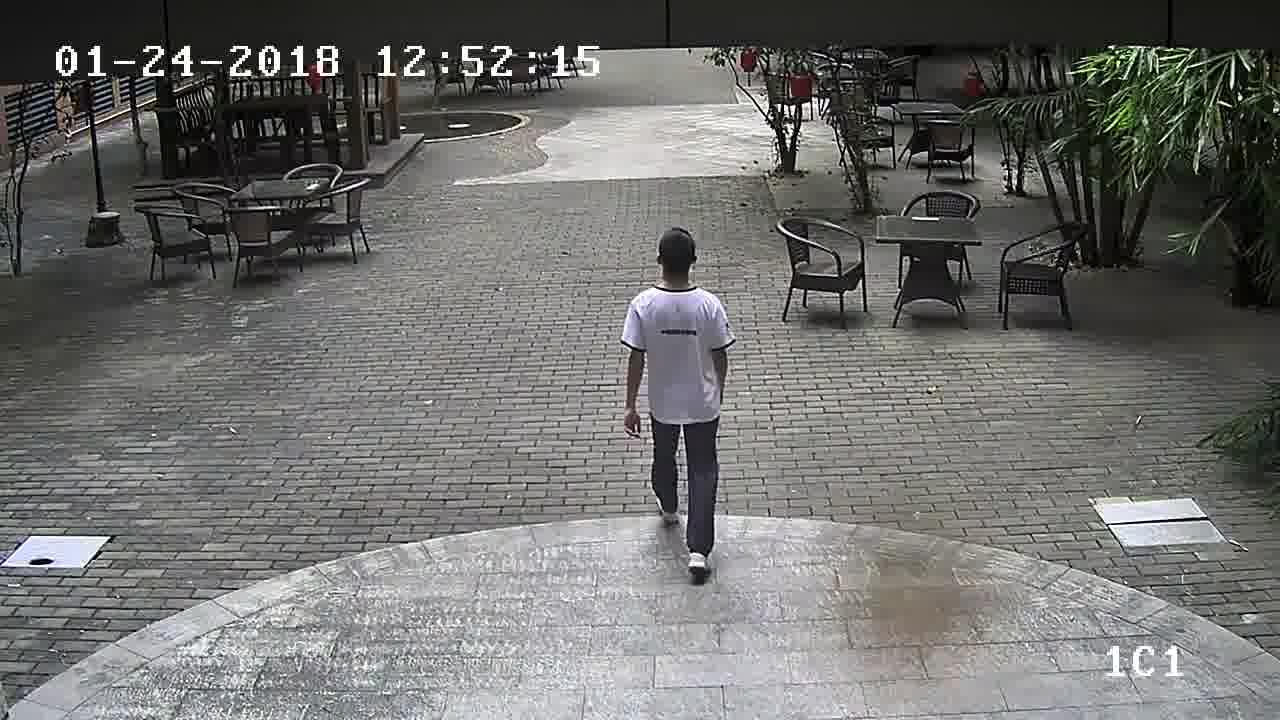
\includegraphics[width=0.3\textwidth]{figures/1-4}\\
            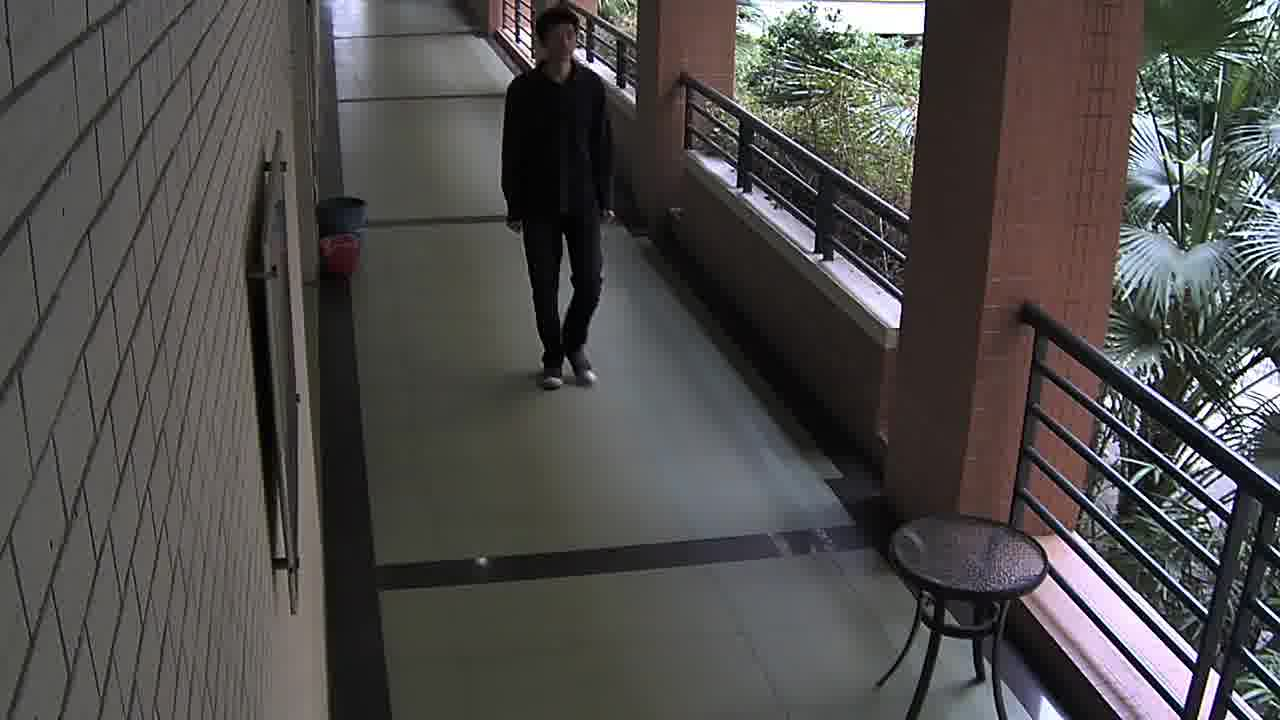
\includegraphics[width=0.3\textwidth]{figures/2-3}
            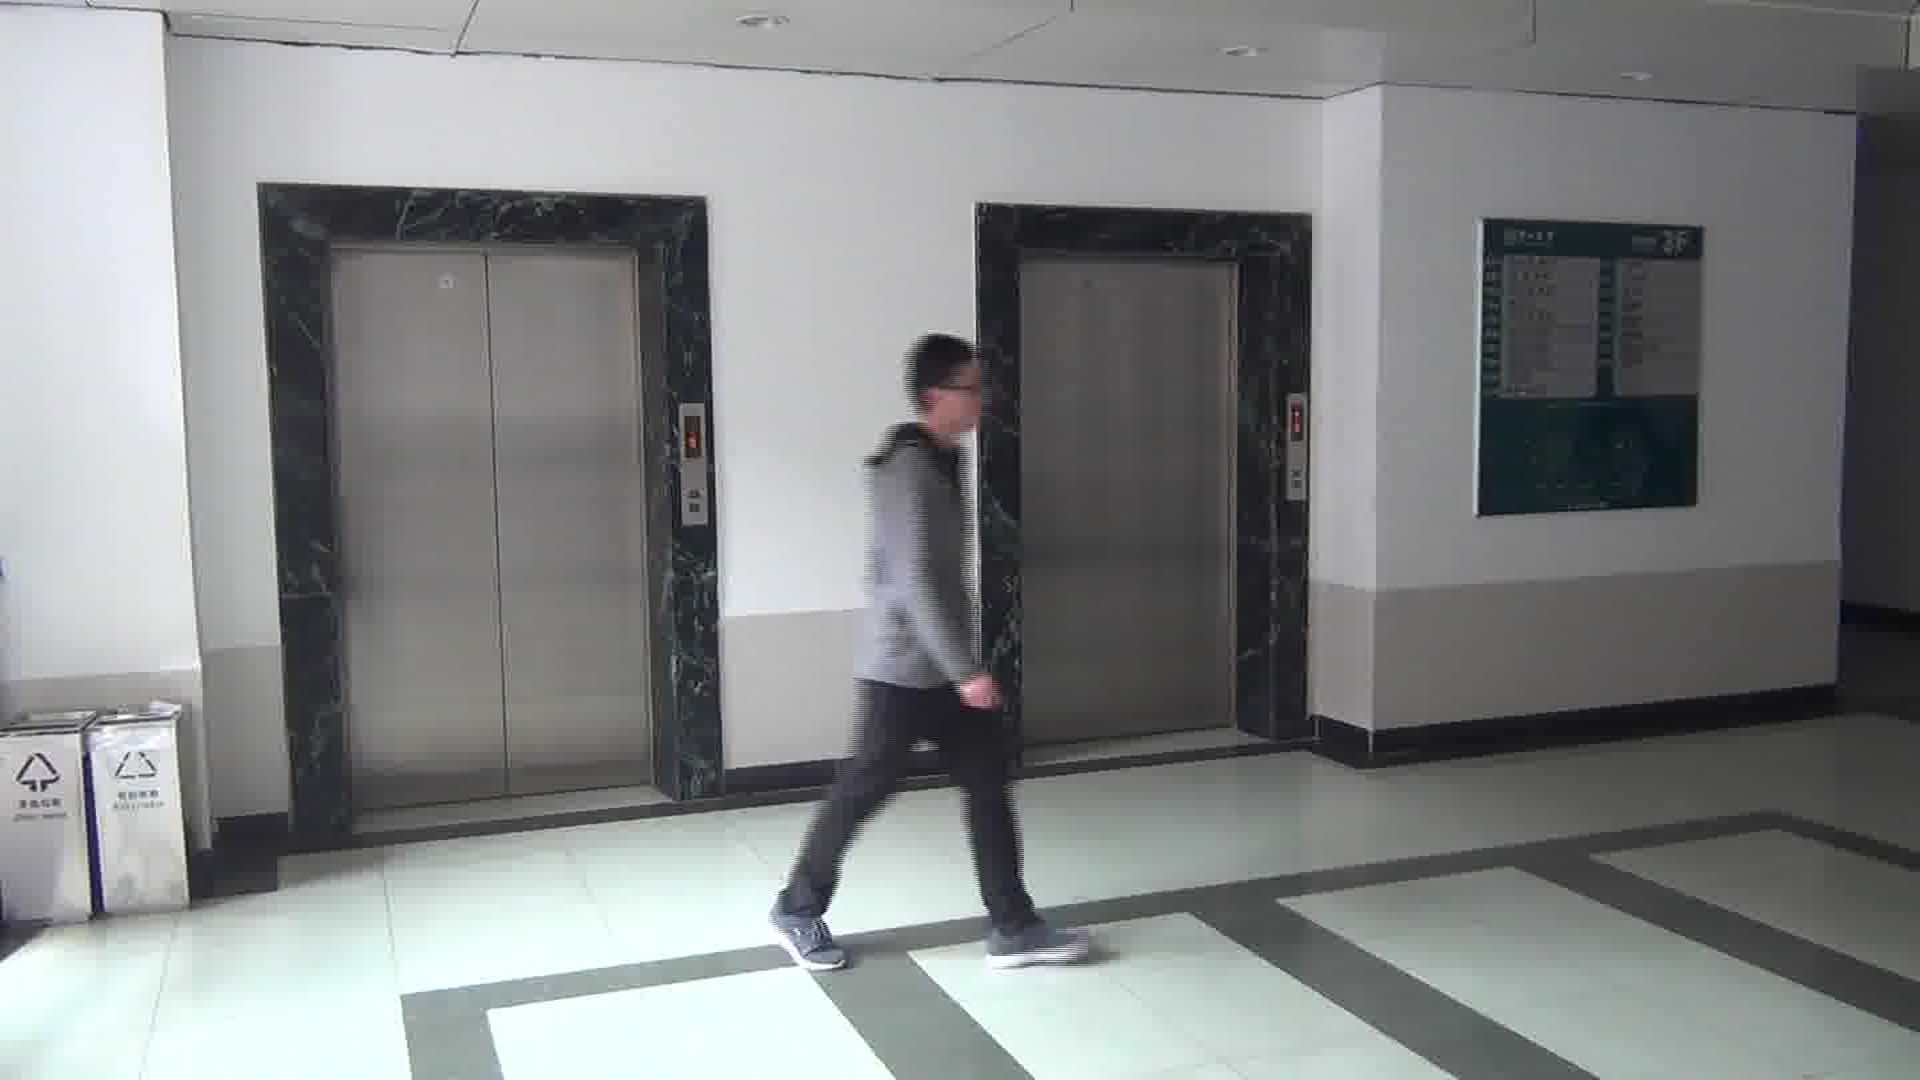
\includegraphics[width=0.3\textwidth]{figures/3-2}
            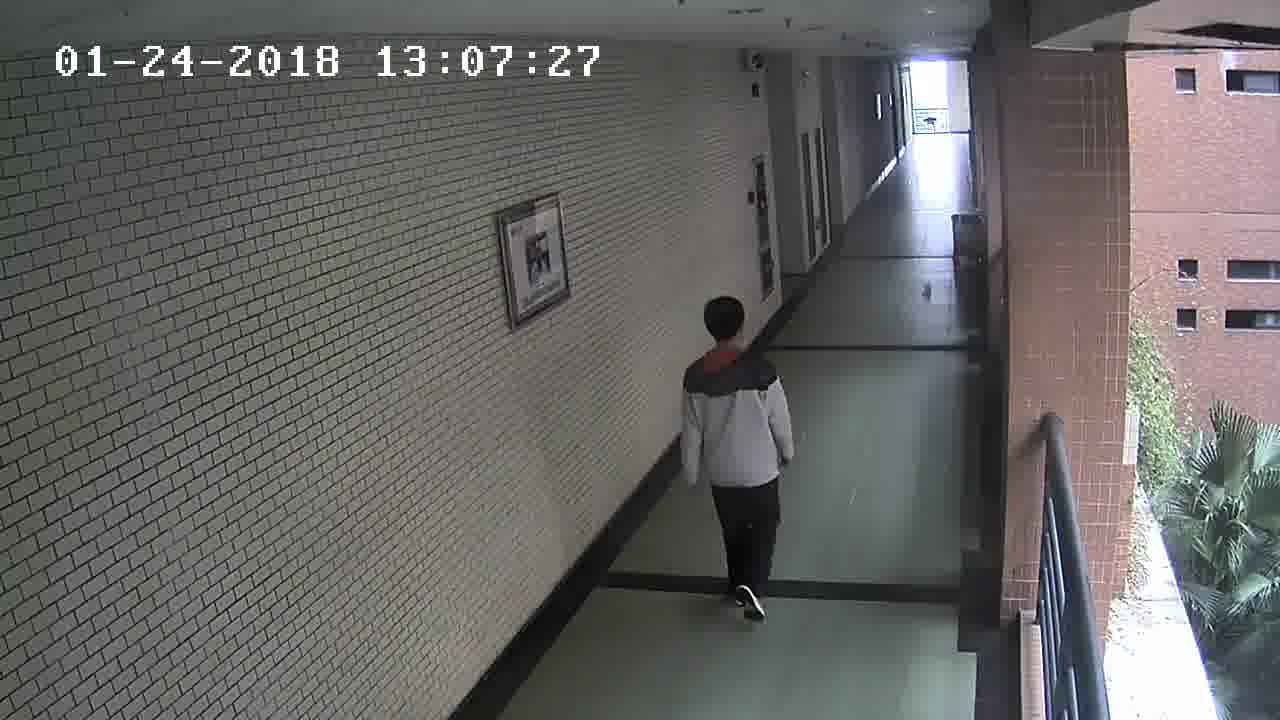
\includegraphics[width=0.3\textwidth]{figures/3-6}
            \caption{最优部署方案}
            \label{fig:rlresult}
            \end{figure}
        \end{column}
    \end{columns}
    \end{frame}


\section{理论框架}
项目的理论框架主要包括当前行人重识别领域state-of-the-art的算法思想、摄像头部署方案的评价指标以及强化学习模型在项目中的应用。

\subsection{行人重识别领域state-of-the-art的算法思想}

\subsubsection{Part-based Convolutional Baseline (PCB)}
这篇论文的Baseline采用了最近很热门的Part的思想,但不同于计算图片中的Attention,而是简单地将图片在垂直方向上分块,获取每一个块的特征。

图\ref{fig:baseline} 是Baseline的架构图。在Baseline中,模型以ResNet50作为Backbone Network。ResNet50模型首先在ImageNet数据集上训练至收敛,然后去掉为ImageNet分类任务而设计的全局池化层(Global Average Pooling Layer)及其后面的全连接层(Fully Connected Layer),使ResNet50模型成为一个高效的图像特征提取器,其中的特征既包括颜色、纹理、形状等视觉特征,也包括类别、姿势、性别等语义特征。作为一个端到端(End-to-End)的特征提取器,其输入为包含RGB通道的原始图像,输出为包含2048个通道(2048 Channels)的Feature Maps。

将ResNet50模型输出的Feature Maps在竖直方向上分成$p=6$个水平条(Horizontal Stripes),每个通道(Channel)保持独立。每个水平条通过一个尺寸与水平条尺寸相同全局池化层,使得原本为矩形的水平条变为一个$1\times1$的像素点,再将其与同一水平条其他通道的像素点拼接起来得到一个$2048\times1\times1$的向量。因为每个水平条会得到一个特征向量,所以经过全局池化层之后可得到$p$个向量,每一个向量都能表示原图像在对应的水平条范围内的局部特征。此方法的优点是简单、高效、易实现,缺点是每个人各部位的分布不同,人物上所具备的关注点也千差万别,将Feature Maps在竖直方向上均匀分割不能很好地体现人与人之间的这些差异。

得到$p$个2048维的特征向量之后,再使用核尺寸为$1\times1$的卷积层将每个2048维的向量降为256维,以减少之后分类任务的计算量。每一个局部特征向量后接一个$n$分类器以预测该图像的类别,其中$n$为训练集中label的个数。训练的损失函数(Loss Function)使用交叉熵损失(Cross Entropy Loss)。

在测试阶段,也即特征提取阶段,将最后的$p$个$n$分类器去掉,直接将$p$个256维的向量拼接(concatenate)为向量$\textbf g$或将$p$个2048维的向量拼接为向量$\textbf h$作为原始行人图像的特征表示。

\subsubsection{Refined Part Pooling (RPP)}
Part-based Convolutional Baseline (PCB) 将Feature Maps在竖直方向上均匀分成$p$个水平条,以获得行人各部位的特征。此方法有操作简单、运算量少、易于实现的优点,但忽略了人与人之间各部位的位置差距。因此,有必要在Baseline的基础上进行改进,不再局限于一个规范的矩形,而是通过计算判断每一个像素点「应该属于」哪一个部分。对于不同通道、相同位置的像素点,进行统一处理。

于是目标就成了:给定一个列向量(column vector,表示不同通道、相同位置的像素点),判断其属于哪一个部分。这就变成了一个分类问题。在这里使用一个线性神经网络层,来将所有的列向量分类。线性神经网络层有权重$W$和偏置$b$组成,为了简化表示,这里省略偏置$b$。对于一个列向量$f$,其属于第$i$个部分的概率$P(p_i|f)$为:
\begin{equation}
P(p_i|f)=\mathop{\rm softmax}\left(W_i^{\rm T}f\right)=\frac{\exp\left(W_i^{\rm T}f\right)}{\sum_j^p\exp\left(W_j^{\rm T}f\right)}
\end{equation}
其中$p_i$表示Feature Map的第$i$部分。

在PCB中,列向量$f$只绝对的属于某一个部分。在求得$P(p_i|f)$后,则可将原始的列向量$f$按照概率分布分配到各部分。对于第$i$个部分$p_i$,其计算方式为:
\begin{equation}
p_i=\frac{1}{H\times W}\sum_{j=1}^{H\times W}P(p_i|f_j)\times f_j
\end{equation}
其中$H$、$W$分别代表Feature Map的高和宽。

如图\ref{fig:refined}所示。

完整的PCB+RPP架构图如图\ref{fig:structure2}所示。

\subsection{摄像头部署方案的评价指标}

\subsection{强化学习模型}

\subsection{面向CPU集群的分布式深度学习训练框架}

\begin{figure}
\centering
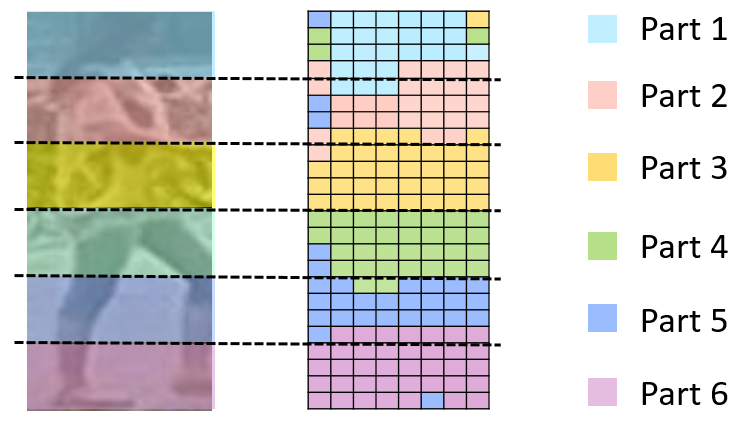
\includegraphics[width=0.6\textwidth]{figure/outliers1}
\caption{Refined Part Pooling示意图}
\label{fig:refined}
\end{figure}

\begin{figure}
\centering
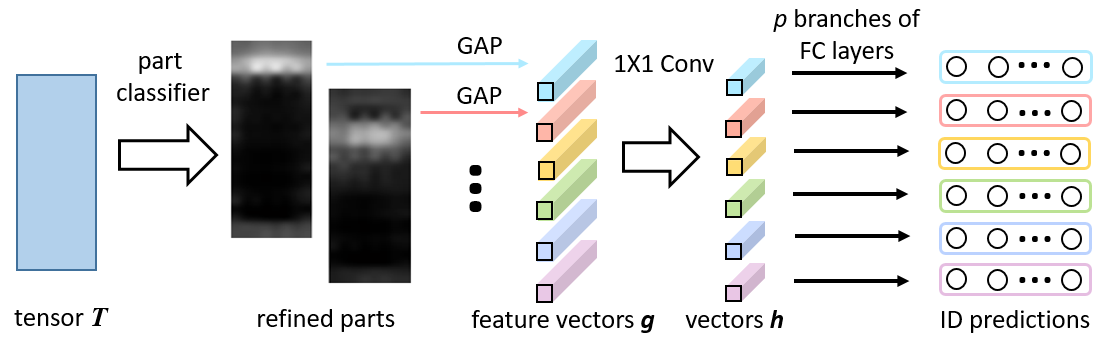
\includegraphics[width=1\textwidth]{figure/structure2}
\caption{PCB+RPP架构图}
\label{fig:structure2}
\end{figure}
\section{项目内容}

\subsection{数据预处理}

\subsubsection{原始视频处理}

\paragraph{视频转码}
原有的摄像头输出的视频文件的时间轴有误,原本时长为 20 分钟的视频却显示有 13 个小时。
部分原始视频文件偶尔会出现一两帧丢失的情况,不是准确的 25 FPS。
原始视频被分割成了 2 $\sim$ 3 个视频文件。
所以需要用 FFmpeg 进行转码。转码保持原有的分辨率不变,填补少量的丢失帧,最终输出正常的视频文件。
此阶段的输出是:每个摄像头对应一个视频文件。

\paragraph{时间点校正和估计}
记录员的对于每一个演员的记录内容为:演员进入视频画面的时间点和演员的标签。将记录员记录的第一个时间点与视频中第一个演员出现的时间点对齐,即可得到每个演员进入视频画面的时间点。
对于那些没有记录员的摄像头,则采用“进入上一个摄像头的时间 + 两摄像头之间平均行走时间”的方法来估计。
由于记录的时候没有精确按照点位进行记录,所以有部分的记录数据需要对照视频重新调整时间点。
此阶段的输出是:每一个演员的进入每一个摄像头的时间点 + 该演员的标签。

\paragraph{视频切割}
有了每一个演员演员进入每一个摄像头的时间点,然后再分别估计每一个摄像头画面中演员停留的平均时间,即可得到每一个演员在每一个视频文件中的时间段,从而利用 FFmpeg 将每一个演员在没一个摄像头的视频片断切割出来。
此阶段的输出是:每个演员在每个摄像头的视频片断。

\subsubsection{行人识别}
行人识别属于计算机视觉领域中的目标识别(Object Detection)问题,目前目标识别问题state-of-the-art 是何凯明等人的Mask RCNN\cite{he2017mask}模型。Mask RCNN在Faster RCNN\cite{ren2015faster}的基础上,添加了一条网络分支,以实现在目标检测的同时,将每个像素分割出来,得到高质量的分割结果。

在本项目中,使用了Mask RCNN作者公开的源代码项目Detectron\cite{Detectron2018}作为行人检测工具,该项目中包含预训练的网络参数和目标检测API,预训练模型在训练过程中使用了COCO 2014\cite{lin2014microsoft}数据集,模型的后端深度神经网络使用了ResNet-101\cite{he2016deep}网络。

对于每个视频文件,遍历其所有的画面帧,调用Detectron API检测画面当中的行人,再根据记录员的记录得到画面中行人的标签。由于画面中可能存在多于一个行人,所以此步骤会将不属于演员的路人也打上演员的标签,需要后期的修正。对于画面中的每一个行人,输出一条记录,其包含的字段分别为:摄像头ID、演员ID、当前帧数、当前帧内行人个数、Bounding Box的左上角与右下角坐标、行人的概率。

\subsubsection{人工标记行人的标签}

由于 Detectron 无法区分在同一帧内的演员和路人,暂时输出了相同的标签,所以需要进一步地用人工把那些路人的标签标记为 -1。

人工标记的过程借助了事先实现的行人重识别baseline,具体过程如下:

将记录中当前帧内行人个数为1的记录挑选出来并按照标签分组,由于该帧中行人数量为 1,所以基本可以确定标签的正确性。把每个 Bounding Box 输入行人重识别 baseline,得到该人的特征。再求标签相同的特征的均值,得到可以代表每一个演员的特征向量。

对于记录中当前帧内行人个数大于1的部分,按照摄像头ID、标签、当前帧数分组,每一组内就是同一摄像头下同一帧内的所有行人的记录。计算每个行人的特征向量与该标签演员的特征向量之间的距离,将距离最近的那条记录的标签标记不变,其它记录的标签改为-1。此时每一个当前帧内行人个数大于1的组内只有一条记录的标签不为-1。

将每个组内标签不为 -1 的图像输出文件,摄像头ID及标签相同的图片放入同一个文件夹,人工评估每个文件夹内的标注结果。删除标注出错的图片,剩余的图片最能代表该场景、该演员的特征,所以求该文件夹内剩余图片的特征向量的均值,作为代表该演员在该场景下的特征向量。

扫描每个文件夹内缺失的图片(文件缺失代表在上一步被删除了,自动标注出错,需要进一步标注),按照与之前步骤类似的做法,找出与对应文件夹内特征向量最近的记录,将其它记录的标签标记为 -1,再次输出图片到文件,人工检查结果。

将每个文件夹内标注出错的结果人工删除。用代码扫描被删除的图片,将原始记录中该帧图像中所有的记录删除。因为到此步骤标注出错的情况很少,所以仅删除了少量的记录。

\subsection{行人重识别领域state-of-the-art论文复现}

\subsubsection{读入训练/测试数据}
Market1501数据集的格式是原始的JPG图片,所以需要加载自己的训练集,这种情况下最好还是继承 Dataset 类比较方便。

Dataset 类的本质是定义了数据所在的位置,以及数据需要预处理的方法。至于数据的位置是在硬盘里面还是提前加载到内存里面,由该类的内部实现决定。由于Market1501数据集过大,所以本项目采用了分批次读取的做法,在训练和测试过程中使用20个进程将数据从硬盘加载到内存中。

\subsubsection{模型训练}

在本项目中,模型的训练使用了Market1501\cite{zheng2015scalable}数据集,数据集使用了水平平移翻转和正则化作为数据扩充的方法。训练模型分为三个阶段,第一阶段是标准的PCB训练,即均匀地分割Feature Map的各个部分。此阶段一共包含60个Epoch,Batch Size为64,模型新增的卷积层的参数初始化为服从正态分布$N(0, 0.001^2)$的随机数。ResNet50网络参数的学习率为0.01,其它参数的学习率为0.1,当Epoch大于或等于40时,各学习率分别缩小为初始的$1/10$。训练模型的第二阶段将PCB中均匀分割改为分类,并且固定第一阶段训练的所有参数,只学习分类层的参数,训练的Epoch数和Batch Size与第一阶段相同。分类层的参数同样初始化为服从正态分布$N(0, 0.001^2)$的随机数,初始学习率为0.01,当Epoch大于或等于40时,学习率缩小为初始的$1/10$。训练模型的第三阶段为调整整个网络中所有的参数,训练的Epoch数和Batch Size与第一阶段相同。所有参数的初始学习率为0.01,当Epoch大于或等于40时,学习率缩小为初始的$1/10$。

\subsubsection{特征提取}

在特征提取阶段,将最后用于分类任务的全连接层移除,并将全连接层移除后网络最后一层或倒数第二层输出的$p$个向量拼接起来,得到行人的特征表示。在测试阶段,采用欧氏距离衡量各特征之间的相似度。

\subsection{强化学习框架实现}

强化学习框架实现了Q-Learning算法以及监控摄像头部署方案评价指标计算函数。在Q-Learning算法中,智能体的生命周期数$N$为100000,状态的长期价值$Q$的学习率$\alpha$为0.01,智能体的远见性$\gamma$为0.2。

\subsection{面向CPU集群的分布式深度学习训练框架}

若要使用分布式训练,需要初始化各节点与master节点的通信连接,然后等待master节点发来的训练任务。

\section{实验过程与结果}
\subsection{实验过程}
实验环境为天河二号的GPU分区,一共使用了4个节点,每个节点配有NVIDIA Tesla K80显卡,
显卡的RAM为11GB,支持单机多卡运算。

将写好的代码传入天河二号中转机,然后为每个节点创建作业进程,每个进程除了rank不一致外,
其它部分都相同。

创建作业之后可以使用yhq命令查看当前作业队列的执行情况。如下图所示。从图中可以看到当前
一共有5个作业正在执行,执行的分区是天河二号的GPU分区,作业的脚本名称为reid.sh,当前的
状态是R,代表着正在运行,作业已经正常运行了24分钟38秒,每个作业占用了1个节点,节点的
名称分别是gn10 - gn14。\\[0.5cm]
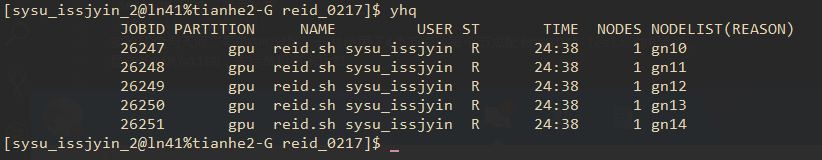
\includegraphics[width=1\textwidth]{figure/yhq}

使用SSH登录计算节点后,可以用top命令查看CPU的占用情况。如下图所示。从图中可以看出
python进程只占用了CPU的10个核心,主要用于训练数据的搬运和预处理,以及各节点之间的通信。
由于训练数据集采用了边用边读的方式,所以内存占用很少。\\[0.5cm]
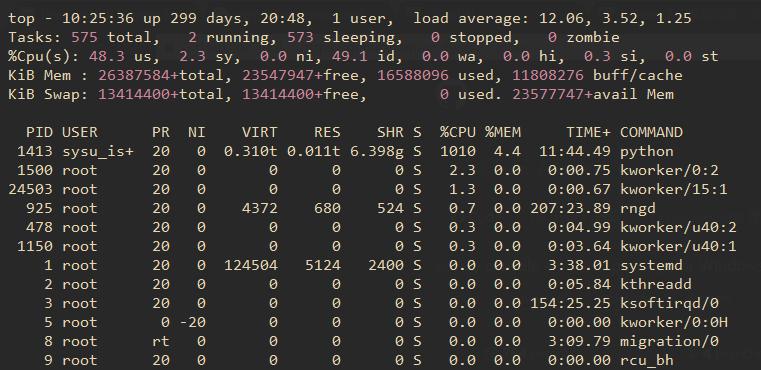
\includegraphics[width=1\textwidth]{figure/top}

使用nvidia-smi命令可以查看GPU的占用情况。如下图所示。可以看到gn10节点有4块NVIDIA Tesla K80
显卡,每一张的显存是11GB,模型的训练进程将4张卡都占用了,正在并行地计算。\\[0.5cm]
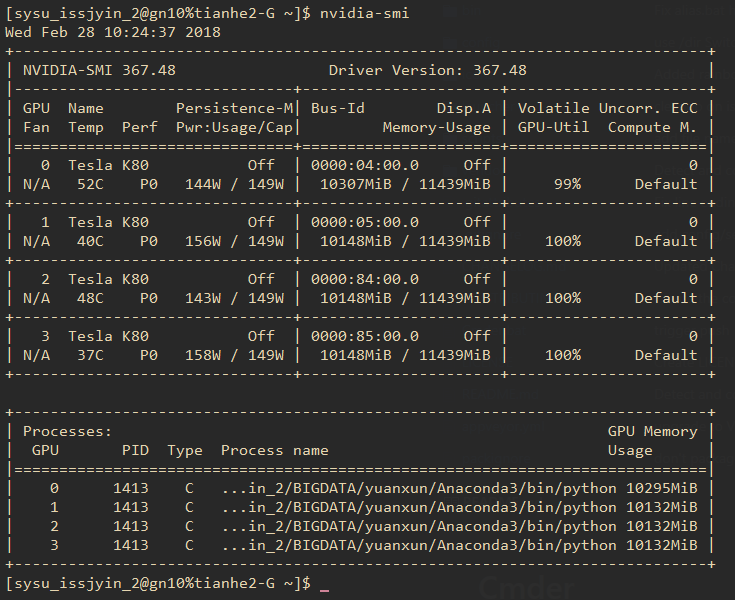
\includegraphics[width=1\textwidth]{figure/smi}
\subsection{实验结果}
\subsubsection{训练}
图\ref{fig:loss}为训练过程的交叉熵误差随着迭代次数的变化曲线:

图例64-5-60表示训练的Batch Size是64,分布式训练的节点数为5,Epoch数为64。需要注意的是,
图中不同节点数的曲线,其训练完成所花费的时间是不一样的,2个节点的训练过程大约需要11个小时,
1个节点的训练大约需要22个小时。从图中可以看到在相同的迭代次数下,节点数越少,误差下降得越快。

其中的原因是,并行训练的原理是将训练数据随机分块并分配给各节点,各节点用该部分数据独立地进行
Forward和Backward操作,计算梯度,最后与其它节点共享梯度,完成参数更新。只使用部分的数据,
计算出来的梯度方向不会比用全部数据计算出来的更准确。虽然大体上梯度下降的方向是没错的,但是使用
分布式训练明显走了很多“弯路”,并且节点数越多,下降的相对速度就越慢。
\begin{figure}
\centering
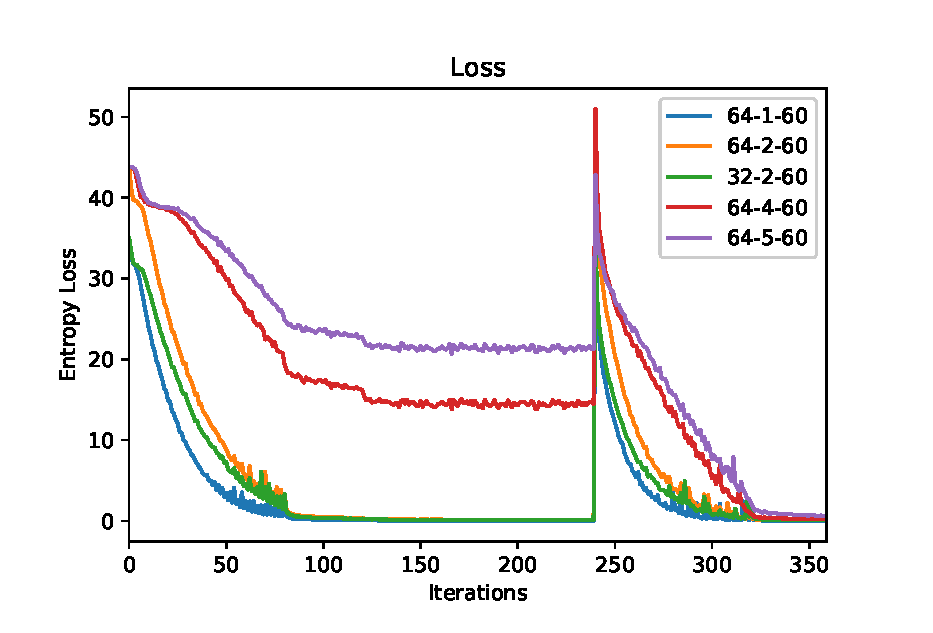
\includegraphics[width=1\textwidth]{figure/loss}
\caption{交叉熵误差随着迭代次数变化曲线}
\label{fig:loss}
\end{figure}
但是在绝对速度的比较上,训练过程所需的绝对时间还是与节点数成反比的,毕竟有更多的节点来分担
计算任务。例如单机训练需要花费22个小时,采用5个节点分布式训练只需要花费5个小时左右。

以上是采用单机训练和多机分布式训练的差异。对于最终训练结果,不管采用单机还是分布式,都会收敛到
一个相近的误差,即虽然过程有差异,但结果差异不大。证明了分布式训练是一种可行的加快训练速度的
方法。

\subsubsection{测试}
表\ref{tab:test}为在Market1501测试集上的测试结果:
\begin{table}[]
\centering
\caption{Market1501测试结果}
\label{tab:test}
\begin{tabular}{@{}lllll@{}}
\toprule
        & Rank1 & Rank5 & Rank10 & mAP  \\ \midrule
64-1-60 & 91.4  & 97.1  & 98.1   & 77.2 \\
64-2-60 & 89.6  & 96.3  & 97.8   & 75.2 \\
32-2-60 & 90.5  & 96.7  & 98.0   & 76.8 \\
64-4-60 & 89.5  & 96.1  & 96.7   & 75.4 \\
64-5-60 & 89.9  & 96.3  & 97.2   & 75.6 \\ \bottomrule
\end{tabular}
\end{table}

可以看出分布式训练结果的精度在误差允许的范围内。

\section{总结}
经过两个月紧张的毕业设计项目,作者在此过程中搭建了PyTorch分布式环境,完成了论文复现工作,在Market1501\cite{zheng2015scalable}数据库上进行实验。实现了 Q-Learning 强化学习算法,选择最优的摄像头部署方案。将深度行人重识别模型的训练算法改造成适用于多CPU集群的形式。

毕业设计的当前进度符合原计划的安排,在接下来的一段时间内应该继续完成剩余的实验项目,以及尽快完成毕业设计的论文写作和文献翻译工作。
%============= 参考文献 =====================
\addcontentsline{toc}{section}{参考文献}
\bibliography{bibfile}


\end{document}
%%%%%%%%%% 结束 %%%%%%%%%%
